%%%------------------------------------------------------------------------------------------------------------
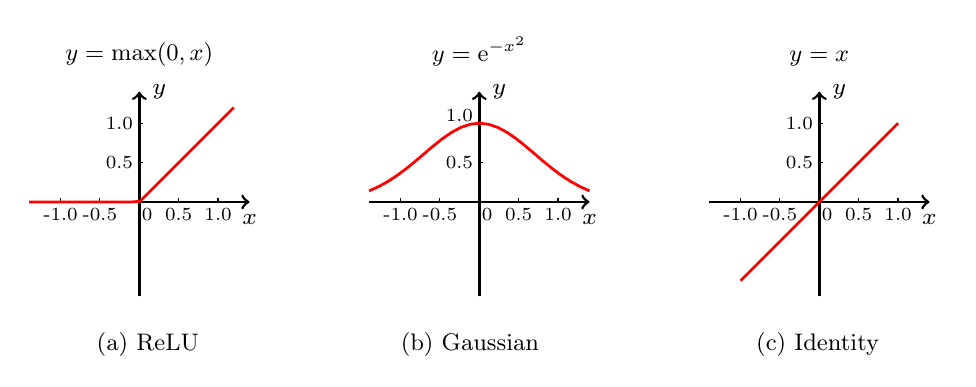
\begin{tikzpicture}
\tikzstyle{every node}=[scale=1.2]
\begin{scope}
  \draw[->, line width=1pt](-1.4,0)--(1.4,0)node[left,below,font=\scriptsize]{$x$};
        \draw[->, line width=1pt](0,-1.2)--(0,1.4)node[right,font=\scriptsize]{$y$};
        \foreach \x in {-1.0,-0.5,0.5,1.0}{\draw(\x,0)--(\x,0.05)node[below,outer sep=2pt,font=\scriptsize,,scale=0.8]at(\x,0.1){\x};}
        \node[below,outer sep=2pt,font=\scriptsize,scale=0.8]at(0.1,0.1){0};

        \foreach \y in {0.5,1.0}{\draw(0,\y)--(0.05,\y)node[left,outer sep=2pt,font=\scriptsize,,scale=0.8]at(0.1,\y){\y};}
        \draw[color=red ,domain=-1.4:1.2, line width=1pt]plot(\x,{max(\x,0)});
        \node[black,anchor=south,scale=0.8] at (0,1.6) {\small $y =\max (0, x)$};
\node [anchor=south east,inner sep=1pt,scale=0.8] (labeld) at (0.8,-2) {\small{(a) ReLU}};
\end{scope}

%%%------------------------------------------------------------------------------------------------------------
\begin{scope}[xshift=1.7in]
        \draw[->, line width=1pt](-1.4,0)--(1.4,0)node[left,below,font=\scriptsize]{$x$};
        \draw[->, line width=1pt](0,-1.2)--(0,1.4)node[right,font=\scriptsize]{$y$};
        \foreach \x in {-1.0,-0.5,0.5,1.0}{\draw(\x,0)--(\x,0.05)node[below,outer sep=2pt,font=\scriptsize,scale=0.8]at(\x,0.1){\x};}
        \node[below,outer sep=2pt,font=\scriptsize,scale=0.8]at(0.1,0.1){0};
        \foreach \y in {0.5,1.0}{\draw(0,\y)--(0.05,\y)node[left,outer sep=2pt,font=\scriptsize,scale=0.8]at(0.1,\y){};}
        \node[left,outer sep=2pt,font=\scriptsize,scale=0.8]at(0.1,0.5){0.5};
        \node[left,outer sep=2pt,font=\scriptsize,scale=0.8]at(0.1,1.1){1.0};
        \draw[color=red ,domain=-1.4:1.4, line width=1pt]plot(\x,{exp(-1*((\x)^2))});
        \node[black,anchor=south,scale=0.8] at (0,1.6) {\small $y ={\textrm e}^{-x^2}$};
\node [anchor=south east,inner sep=1pt,scale=0.8] (labele) at (0.8,-2) {\small{(b) Gaussian}};
\end{scope}

%%%------------------------------------------------------------------------------------------------------------
\begin{scope}[xshift=3.4in]
        \draw[->, line width=1pt](-1.4,0)--(1.4,0)node[left,below,font=\scriptsize]{$x$};
        \draw[->, line width=1pt](0,-1.2)--(0,1.4)node[right,font=\scriptsize]{$y$};
        \foreach \x in {-1.0,-0.5,0.5,1.0}{\draw(\x,0)--(\x,0.05)node[below,outer sep=2pt,font=\scriptsize,scale=0.8]at(\x,0.1){\x};}
        \node[below,outer sep=2pt,font=\scriptsize,scale=0.8]at(0.1,0.1){0};
        \foreach \y in {0.5,1.0}{\draw(0,\y)--(0.05,\y)node[left,outer sep=2pt,font=\scriptsize,scale=0.8]at(0.1,\y){\y};}
        \draw[color=red ,domain=-1:1, line width=1pt]plot(\x,\x);
        \node[black,anchor=south,scale=0.8] at (0,1.6) {\small $y =x$};
\node [anchor=south east,inner sep=1pt,scale=0.8] (labelf) at (0.8,-2) {\small{(c) Identity}};
\end{scope}
\end{tikzpicture}
%%%------------------------------------------------------------------------------------------------------------